In this section the views for a single patient is detailed. It is as earlier described by clicking on a specific patient in either my patients list or all patients list. To go back to the overview the house button which is displayed next to the patients name is clicked. 

\subsubsection{Overview}
\begin{center}
    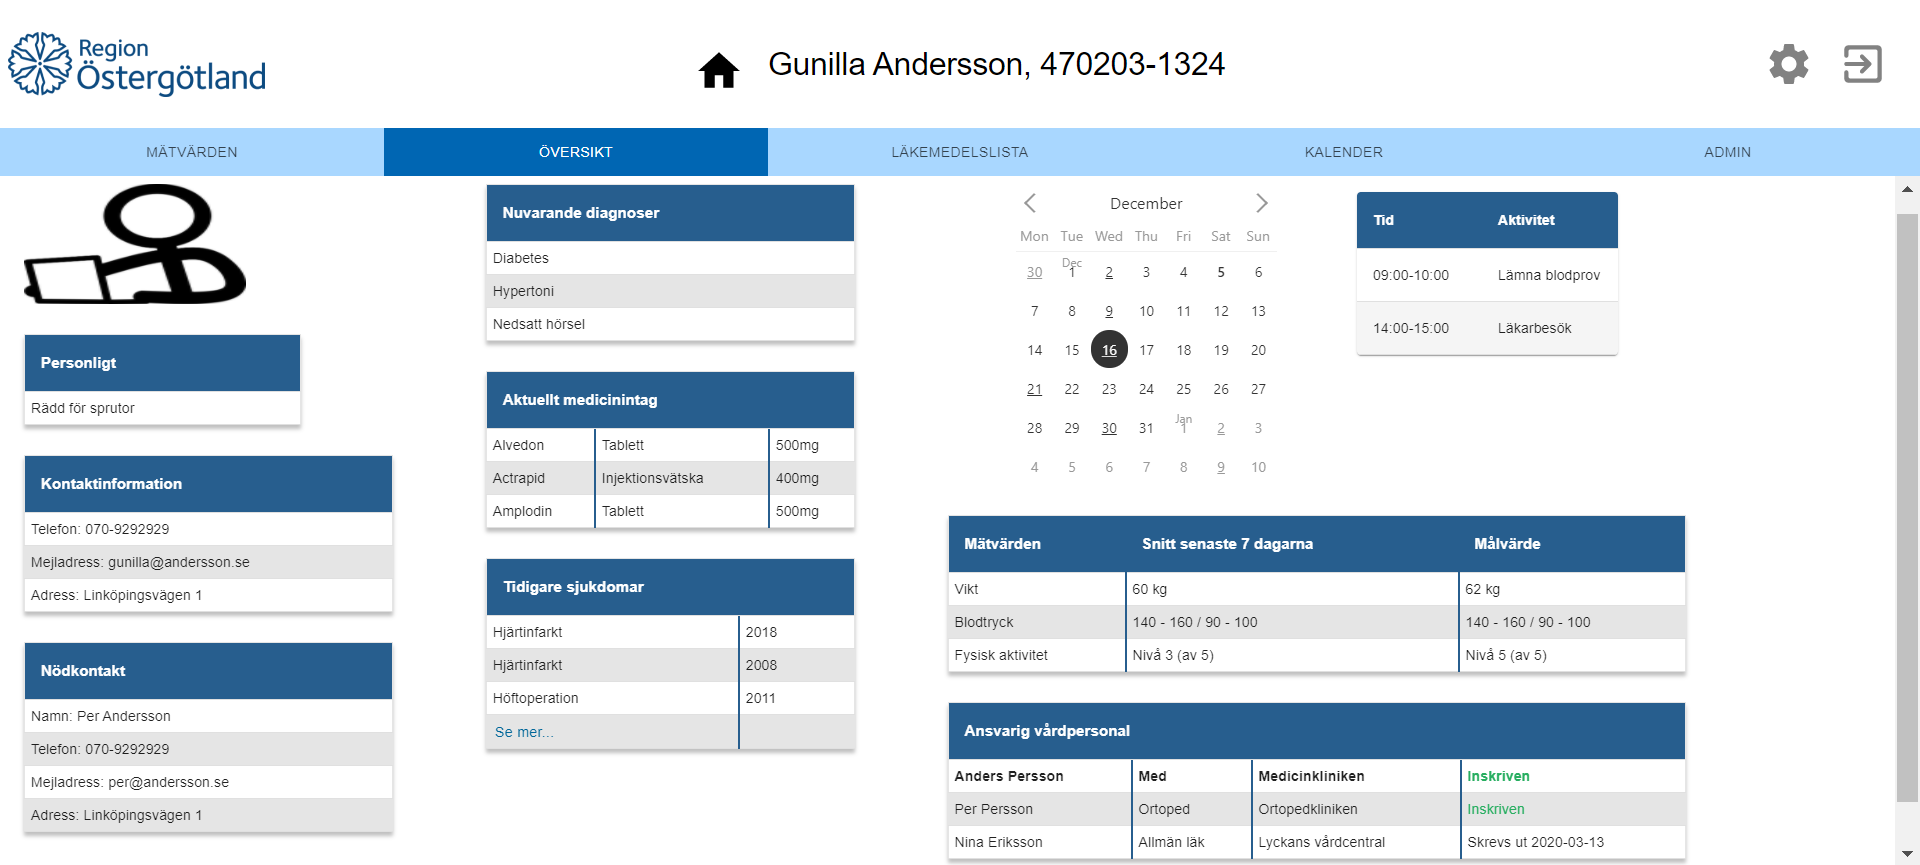
\includegraphics[width=\linewidth]{images/single_patient_overview_image.png}
    \captionof{figure}{Overview single patient}
    \label{fig:figures}
\end{center}
Information about the specific patient with contact information and emergency contact. Shows current diagnoses, current medication intake, average of current measurement values, previous diagnoses and caregivers and staff who handle the patient. Picture of the specific patient. A smaller calendar of the one found in "/patient/calendar" exists as well.

The tables length is adapted to the number of diagnoses, medications, measurements, responsible staff members. 

Table of “tidigare sjukdomar” is shown with a maximum of 4 rows with the see more text included. When pressing see more, the table expands in length and shows the rest of the information.

\subsubsection{Measurements}
    \begin{center}
    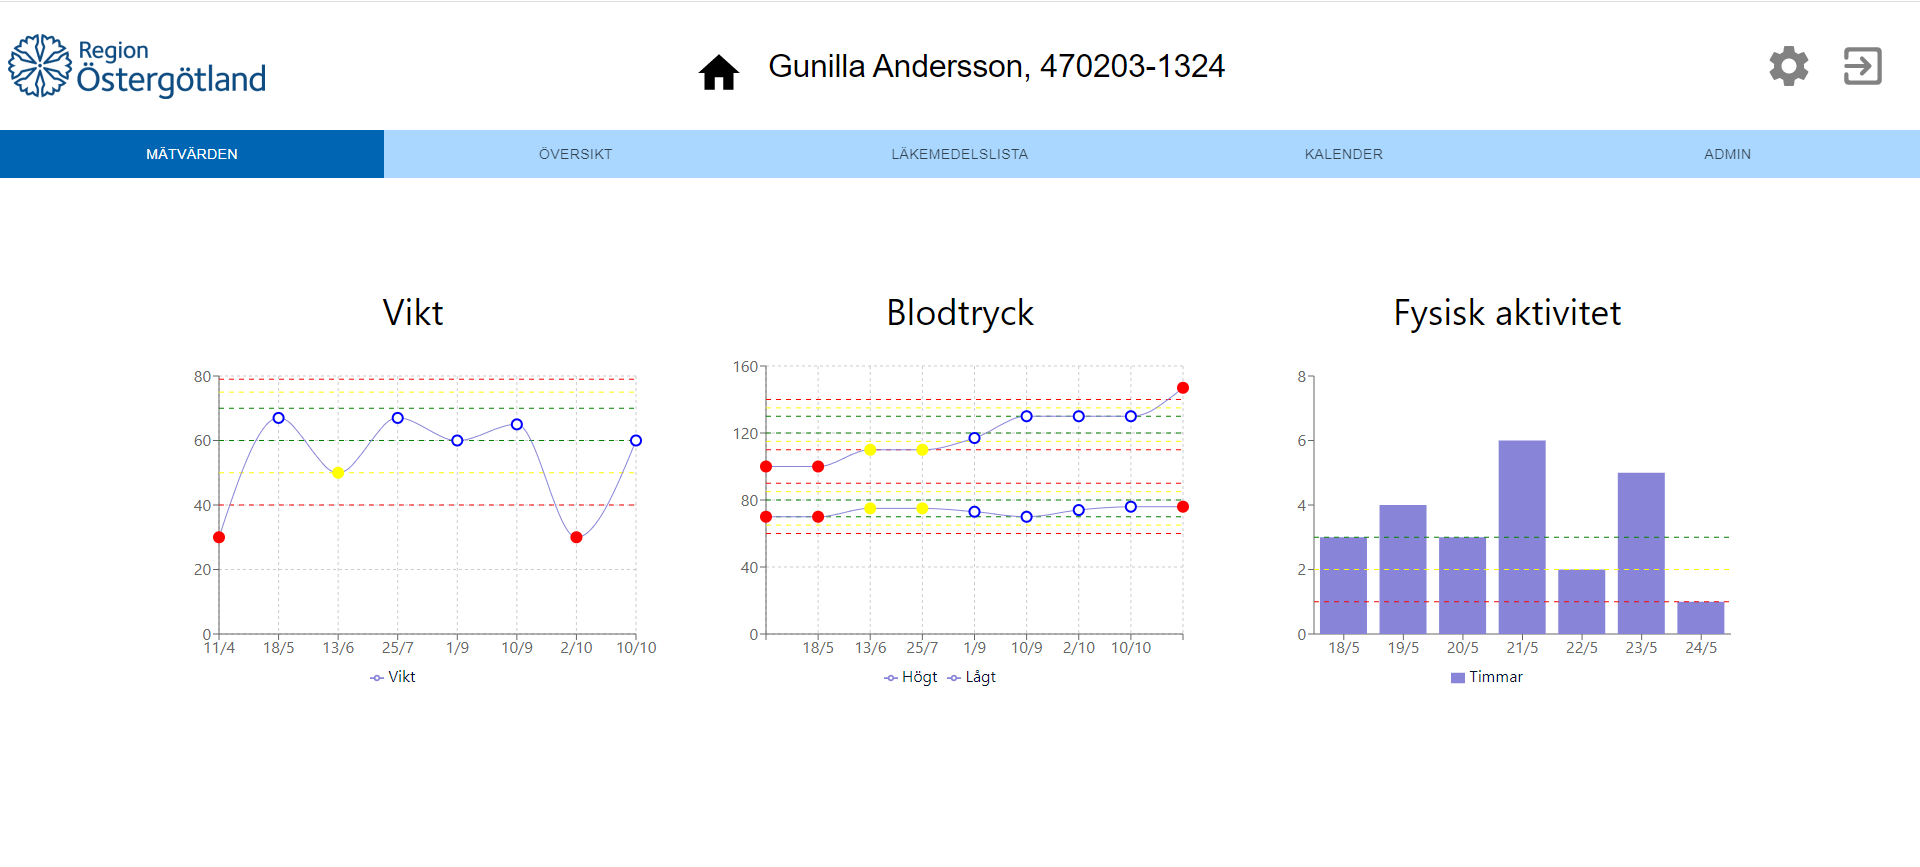
\includegraphics[width=\linewidth]{images/single_patient_measurement_overview_image.png}
    \captionof{figure}{Measurement - overview }
    \label{fig:figures}
\end{center}
All the current measurements for the specific patient are displayed in graphs. In the graph a target range is displayed but also intervals of when a red or yellow warning should be triggered. Measurement points are also seen and if they are outside the allowed references, they become red or yellow depending on severeness. By clicking on a graph you move to the specific measurement were more info and options are displayed
\\

\begin{center}
    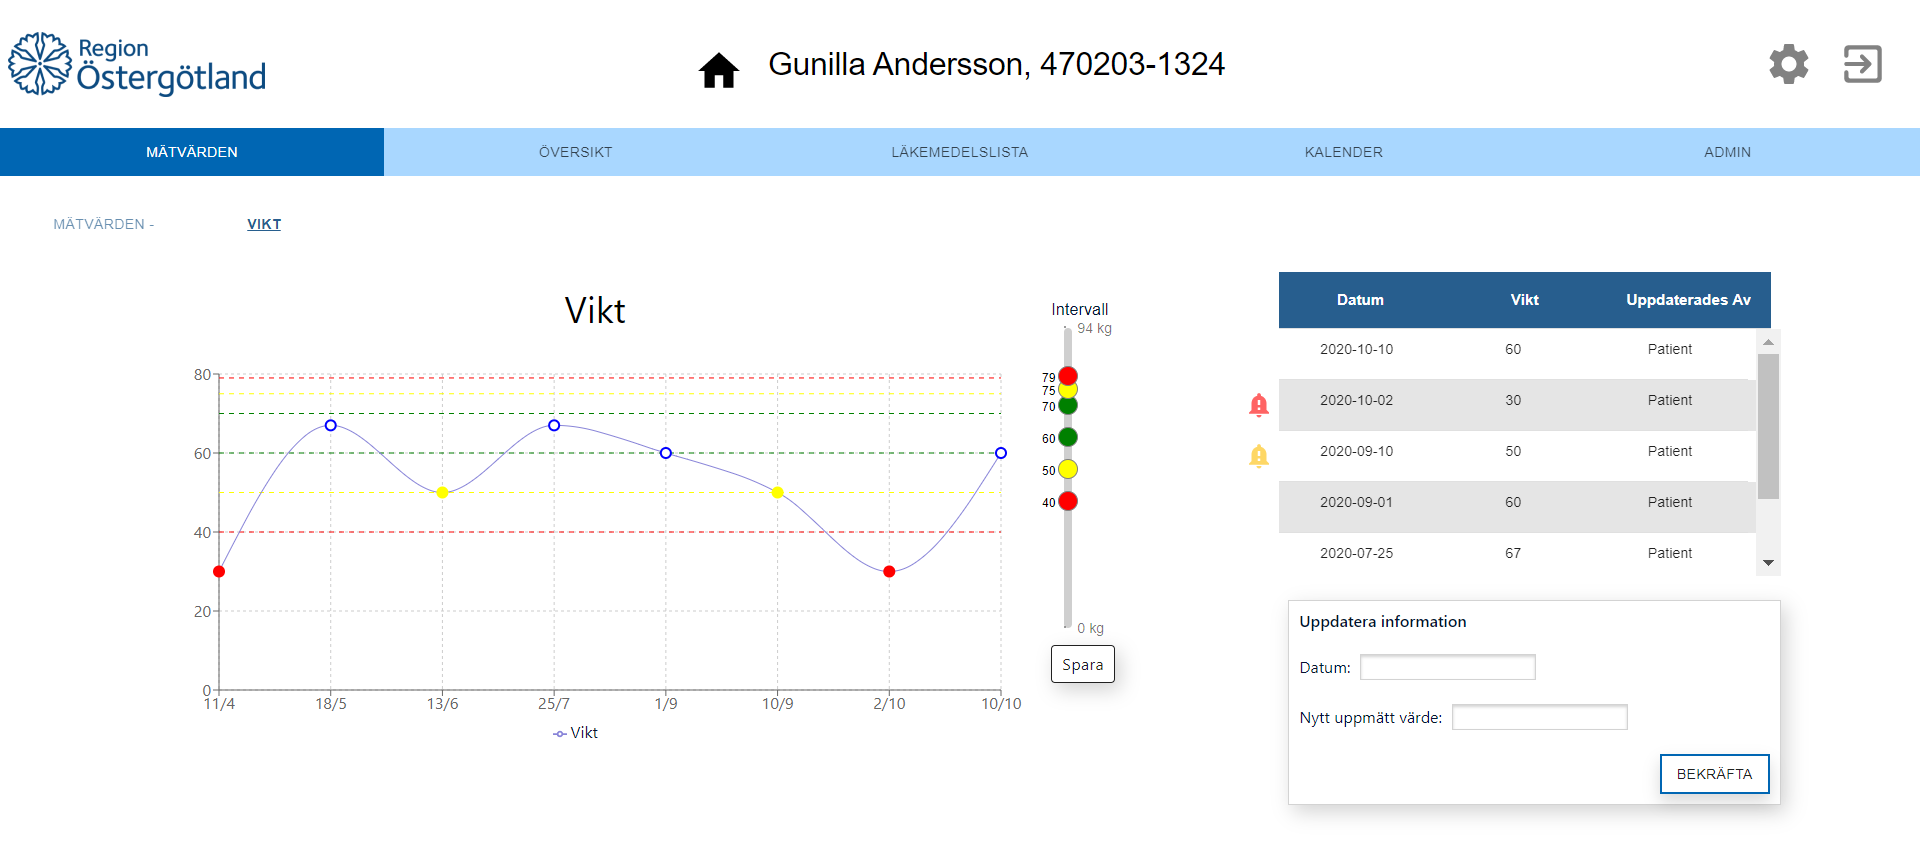
\includegraphics[width=\linewidth]{images/single_patient_weight_measurements_image.png}
    \captionof{figure}{Measurement - single page}
    \label{fig:figures}
\end{center}
On the specific page for a single measurement page, the graph works exactly like before. 

There is also a table at the page were it is possible to click on the notifications for handle the value. When clicking on the notification a pop-up window appears which is described further later. 

----------
\newline
Not fully implemented: 
For admins it is possible to change the reference ranges by moving the green, yellow and red dots displayed to the right of the graph and then click "Spara" (Save). The green dots corresponds to the target value, the yellow to severeness level yellow and the red to severeness level red. 

It is possible to add a new value by filling in the forms "Uppdatera information". Add a date and measure and click on the "Bekräfta" button.
\newline
---------

All the different subpages for specific measurements looks the same, except for that the number of target ranges and reference ranges could vary, for example blood pressure has two, one for systolic pressure and one for dystolic pressure.
\\

\begin{center}
    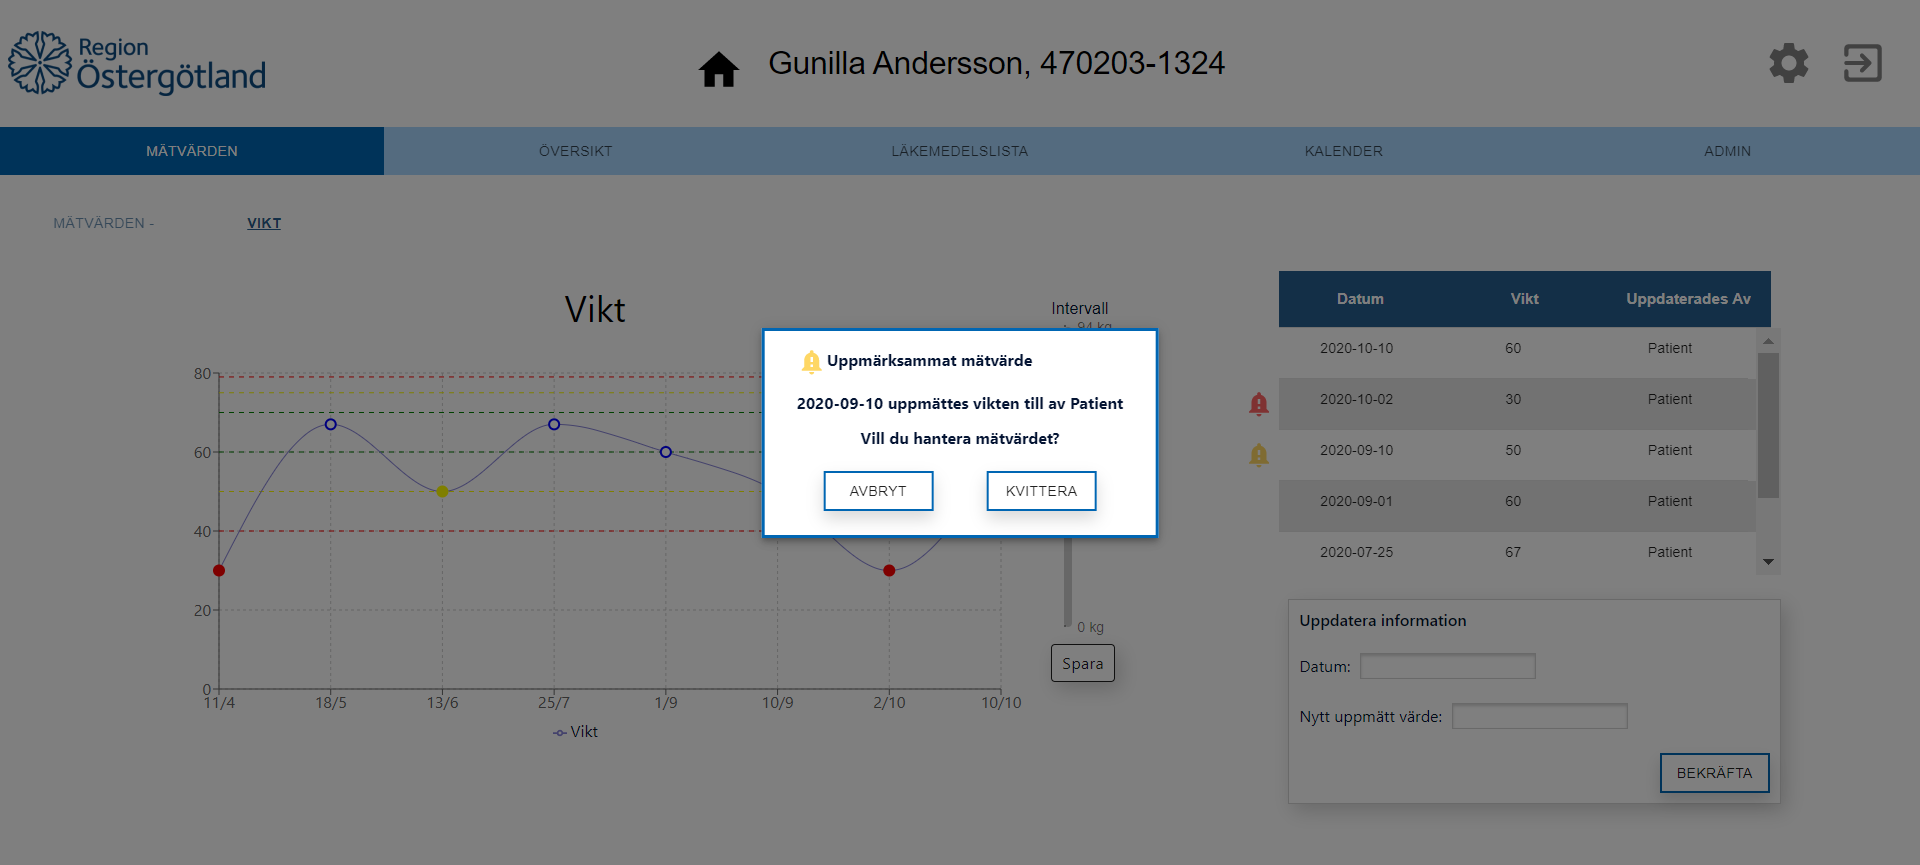
\includegraphics[width=\linewidth]{images/single_patient_weight_measurements_handle1_image.png}
    \captionof{figure}{Measurement - handle change 1 }
    \label{fig:figures}
\end{center}
When clicking on a notification a pop-up window appears with two options, "Avbryt" and "Kvittera". By clicking on "Avbryt" the pop-up window shuts down and nothing happen. By clicking on "Kvittera" another pop-up appears which is described below.
\\

\begin{center}
    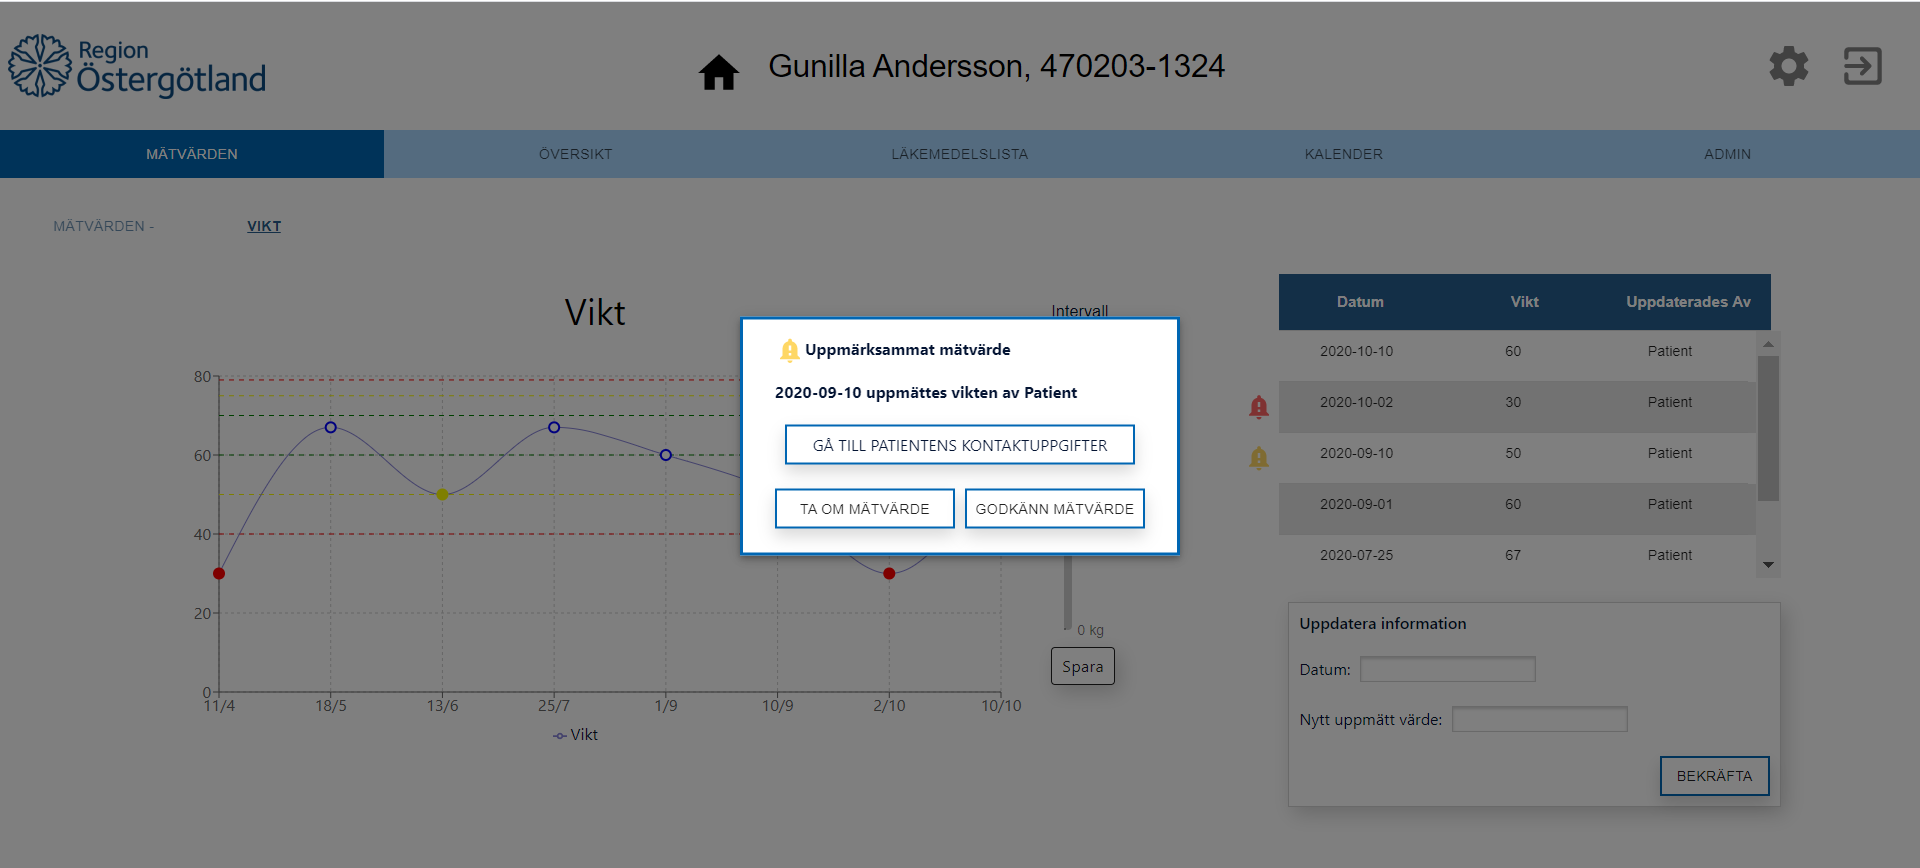
\includegraphics[width=\linewidth]{images/single_patient_weight_measurements_handle2_image.png}
    \captionof{figure}{Measurement - handle change 2 }
    \label{fig:figures}
\end{center}
If clicked on the "Kvittera" button there is now three alternatives. By clicking on "Gå till patientens kontaktuppgifter" you are moved to "patient/overview". By clicking on "Ta om mätvärde" a request is sent to the patient to retake the measured value. By clicking on "Acceptera mätvärde" the notification is taken away.
\\

\subsubsection{Medication list}
\begin{center}
    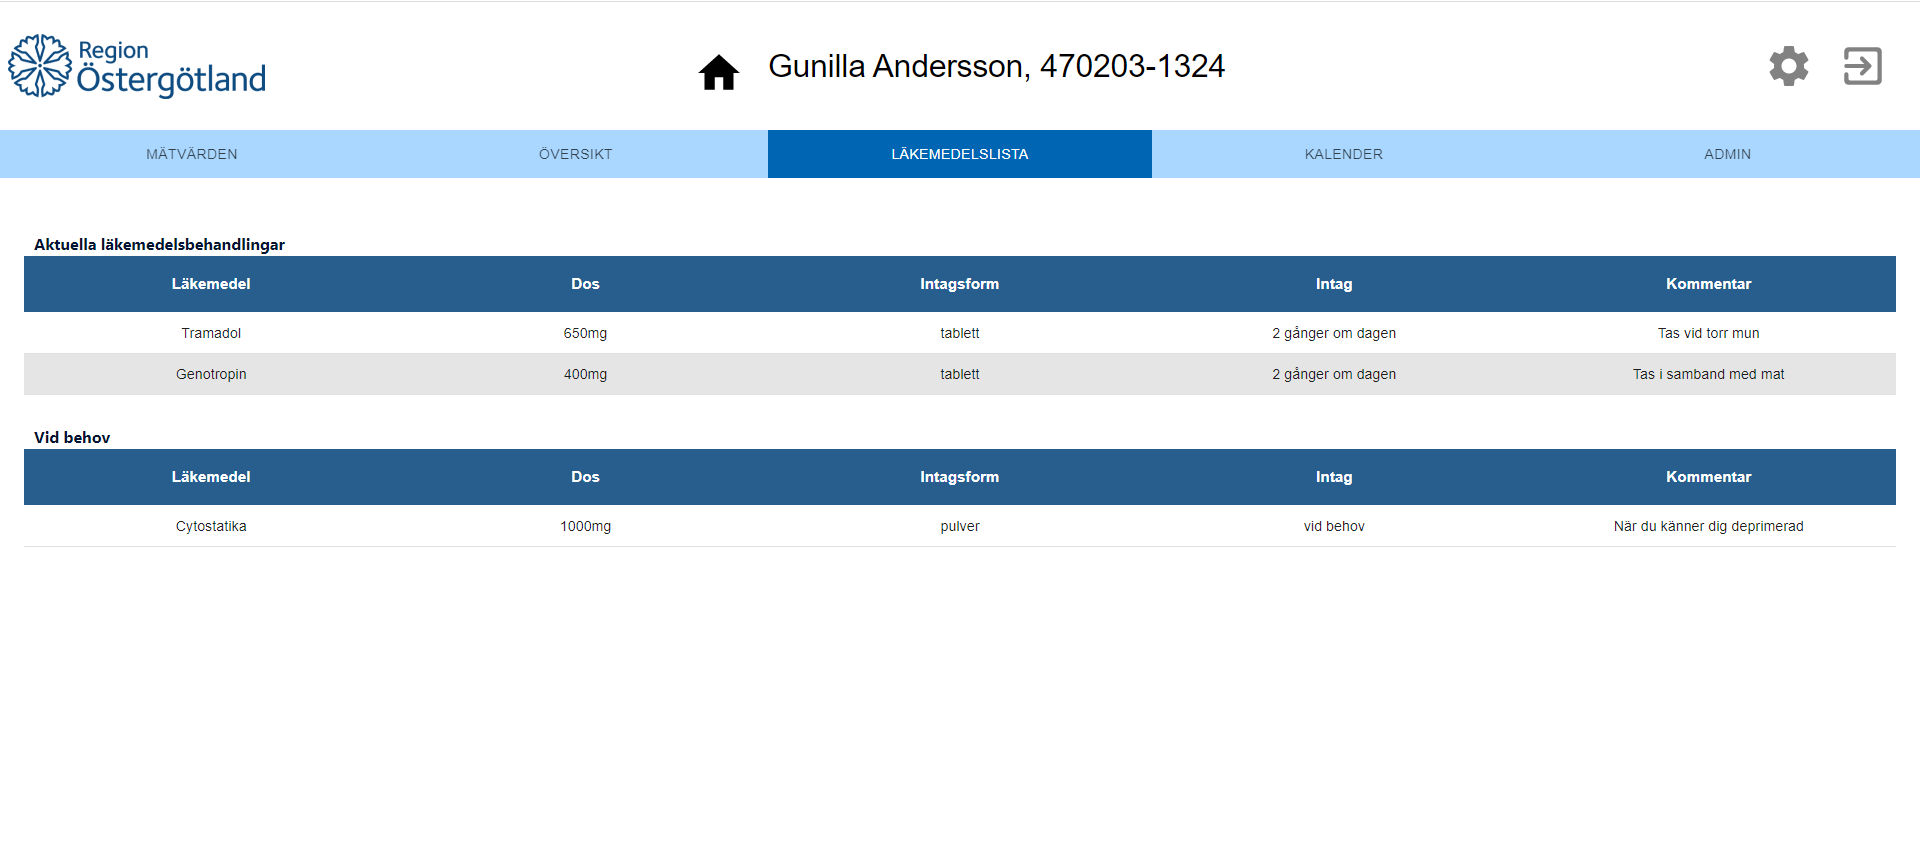
\includegraphics[width=\linewidth]{images/single_patient_medications_image.png}
    \captionof{figure}{Medications}
    \label{fig:figures}
\end{center}
Table of medicines that shows current/relevant medication intake for a specific patient and a table of medicines that a specific patient can take if necessary.
\\

\subsubsection{Calendar}
\begin{center}
    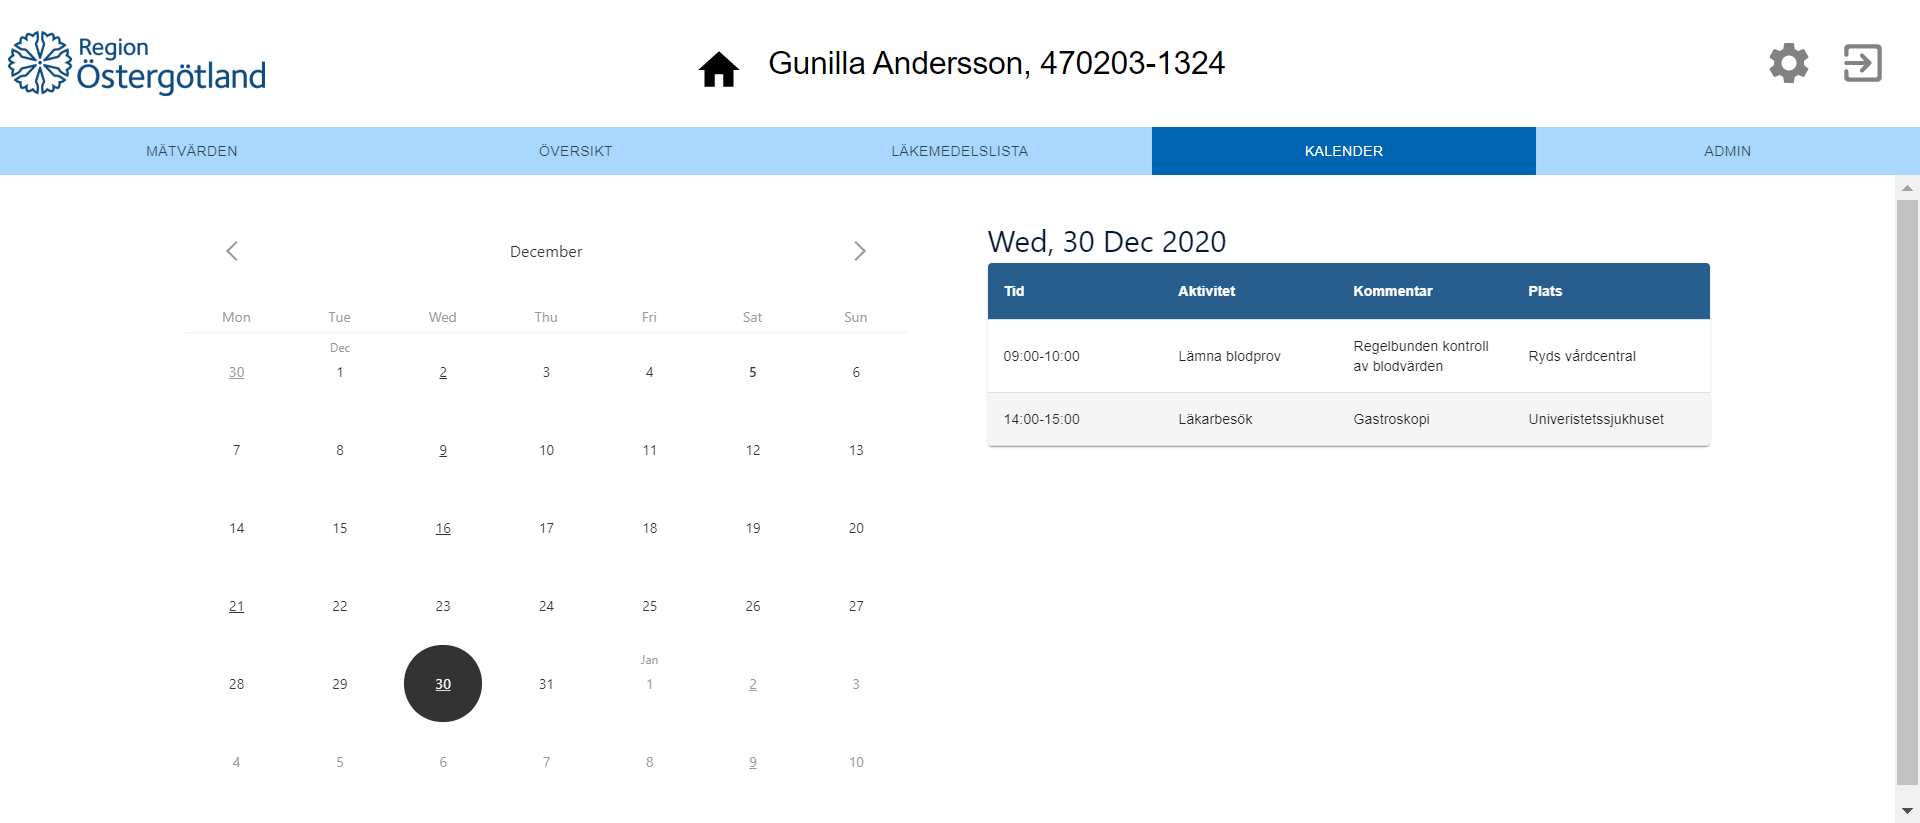
\includegraphics[width=\linewidth]{images/single_patient_calendar_image.png}
    \captionof{figure}{Calendar}
    \label{fig:figures}
\end{center}
As the calendar for all patients but this on does only display the specific patients calendar events.
\\

\subsubsection{Admin}
\begin{center}[h]
    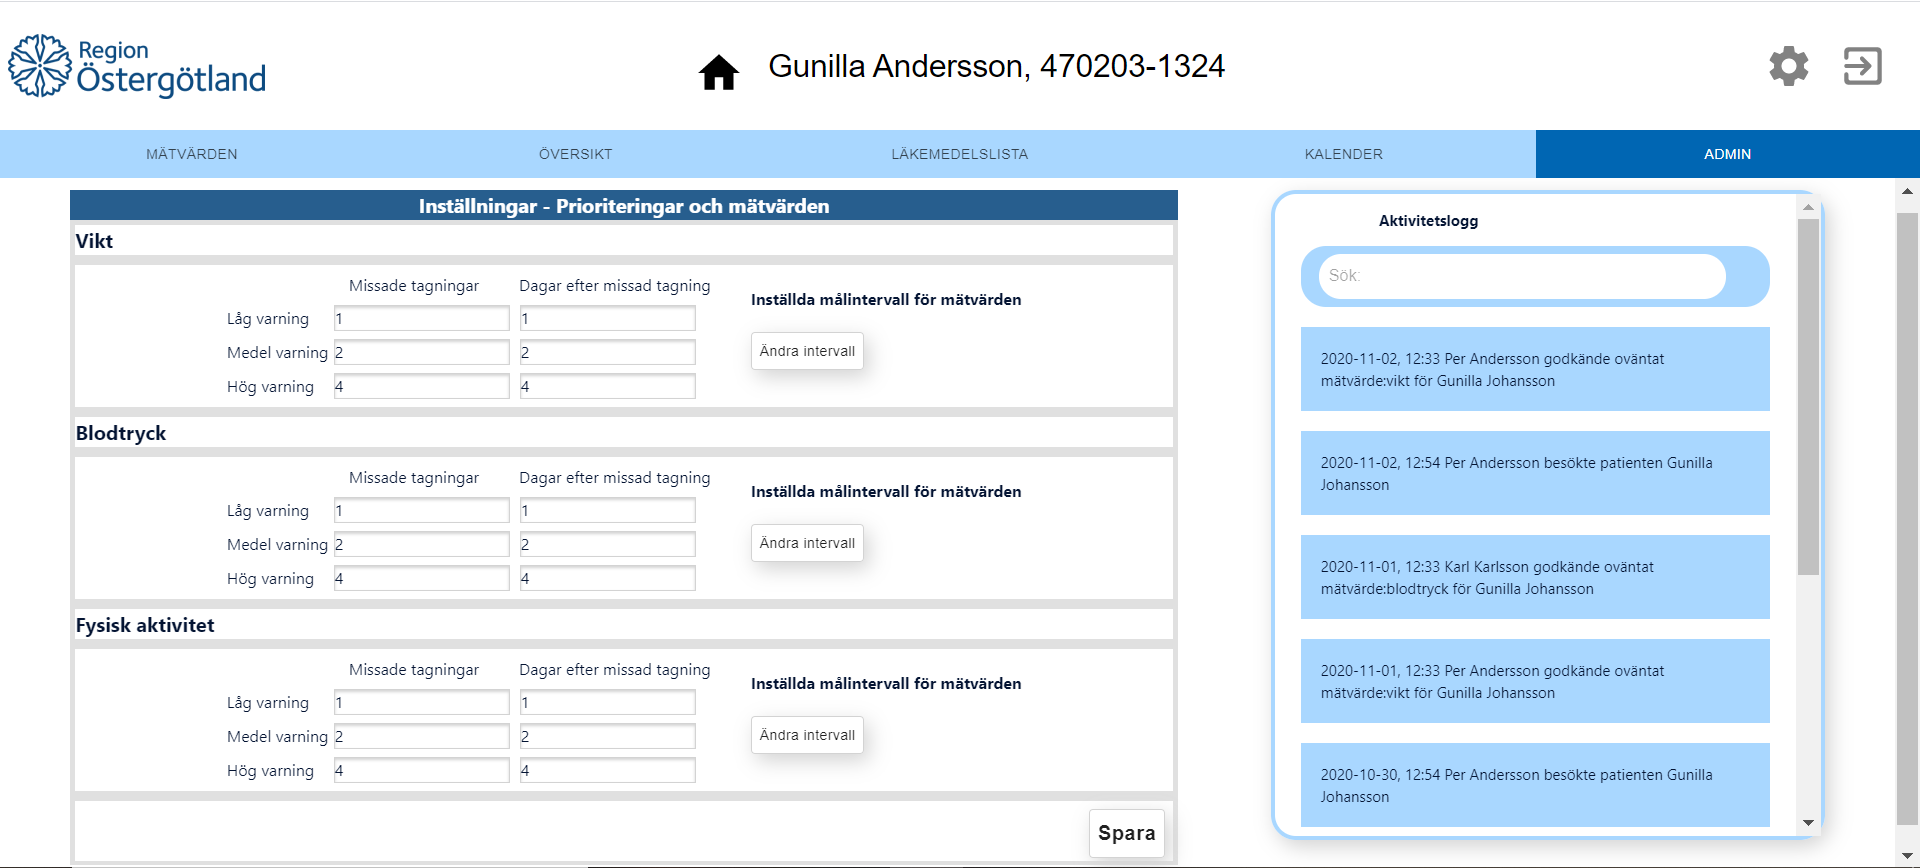
\includegraphics[width=\linewidth]{images/single_patient_admin_image.png}
    \captionof{figure}{Admin}
    \label{fig:figures}
\end{center}
Page only visible for admins. 
Inställningar Prioriteringar Mätvärden:
Set the settings for notifications for the patient measurements. The notifications are rendered by two things, either a measurement which is outside the reference ranges or that the patient have missed to report measurements. 

For changing when a warning should be rendered for missing a measurement, you change in the form for the measurement type and either days without measurement or number of expected measurements not reported, and then click on the "Spara" button at the bottom of the page. 

For changing the target ranges and reference ranges you press “Ändra intervall” and are directed to the measurement page where you can change the interval while seeing the graph at the same time. 

Aktivitetslogg: 
Shows all the activity that happens on a patient specific page. All activities is logged for the patient's integrity.
Not fully implemented: 
The search function. 

\\
